\section{Representación de la imagen analizada}
\label{sec:representacionFiguras}

\gotrev{Última revisión hecha el 20-06-2012}
Tanto en el análisis de imágenes como en el proceso de composición hay un aspecto fundamental a estudiar: la representación de datos de las figuras.\\

De acuerdo con lo explicado en previas secciones, el producto de salida  (y el de entrada de la composición musical) es un archivo XML que almacena el análisis de la imagen dada como entrada. Este archivo contiene toda la información que se considera para representar los elementos de una imagen, y servirá como base para explicar el contenido y estructura lógica de los datos analizados.\\

Por otro lado, en esta sección se mostrará también la estructura usada en la implementación de los Objetos relacionados con estos datos y sus usos. Dado que tanto el módulo de análisis como el de composición hacen uso de esta información , se introducirán también en esta sección las extensiones y capacidades de la estructura de datos creada.

\subsection{Almacenamiento y estructura}
\label{subsec:xmlstruct}

	La información correspondiente a la salida del análisis de imágenes es tal y como muestra la Figura~\ref{fig:estructuraFiguras}. En ella, los nodos están representados por cajas rectangulares, sus atributos con cuadrados y, finalmente, los elementos con círculos. \\

			\begin{figure}[htbp]
			\centering
			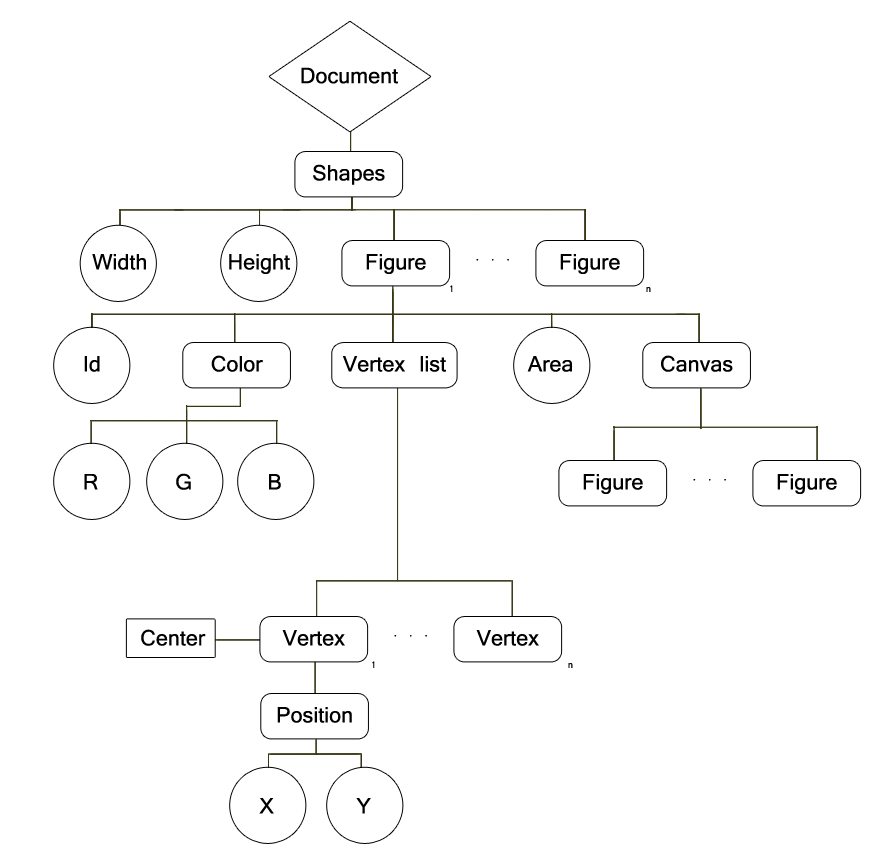
\includegraphics[scale=0.35]{graphics/xml-representation.png}
			\caption{Estructura del archivo xml de análisis}
			\label{fig:estructuraFiguras}
			\end{figure}
		
	La estructura (representada en formato XML) es:\\
	
	\newlist{longenum}{enumerate}{5}
	\setlist[longenum,1]{label=\tiny$\blacksquare$}
	\setlist[longenum,2]{label=\tiny$\blacksquare$}
	\setlist[longenum,3]{label=\tiny$\blacksquare$}
	\setlist[longenum,4]{label=\tiny$\blacksquare$}
	\setlist[longenum,5]{label=\tiny$\blacksquare$}
	
	\begin{longenum}
	\item \textbf{Shapes}: Representa la imagen completa y contiene un listado de las figuras resultantes del análisis.
	\item \textbf{Width}: Almacena el ancho total de la imagen.
	\item \textbf{Height}: Almacena el alto total de la imagen.
	\item \textbf{Figure}: Contiene la información relativa a un polígono en la imagen.
		\begin{longenum}
		\item \textbf{Id}: Identificador único de la figura.
		\item \textbf{Color}: Identificador para almacenar la información sobre el color de la figura.
			\begin{longenum}
			\item \textbf {RGB}: Delimitar la información sobre los valores RGB del color.
				\begin{longenum}
				\item \textbf{R}: Valor referente a la cantidad de rojo en la escala RGB.
				\item \textbf{G}: Valor referente a la cantidad de verde en la escala RGB.
				\item \textbf{B}: Valor referente a la cantidad de azul presente en escala RGB.
				\end{longenum}
			\end{longenum}
		\item \textbf{VertexList}: Lista de vértices que componen el polígono.
			\begin{longenum}
			\item \textbf{Vertex [type=``normal'']}: Identificador para delimitar un vértice que pertenece a uno de los extremos de una recta o curva del polígono.
				\begin{longenum}
					\item \textbf{Position}: Identificador para delimitar la posición de un vértice en la imagen.
						\begin{longenum}
						\item \textbf{X}: Componente x de la posición del vértice.
						\item \textbf{Y}: Componente y de la posición del vértice.
						\end{longenum}
					\item \textbf{Vertex [type=``center'']}: Identificador para delimitar un vértice que señala el centro de circunferencia que forma la curva que conecta el vértice anterior a este con el siguiente.
				\end{longenum}
			\end{longenum}
		\end{longenum}
		\item \textbf{Area}: Valor numérico del área de una figura.
		\item \textbf{Canvas}: Identificador que delimita las figuras situadas dentro de la figura que contiene este elemento. 
	\end{longenum}
	
	Como se puede ver, la imagen analizada está compuesta por una lista de figuras (o polígonos) jerárquicas según su posición geométrica. Cada figura representa una mancha de color detectada por el analizador de imágenes para ello guarda la información de sus vértices, color y área.


\subsection{Vista de Implementación}

	La vista principal de la estructura en un sistema basado en objetos como el tratado se muestra en la Figura~\ref{fig:diagramaClasesFigure}.\\

		\begin{figure}[htbp]
		\centering
		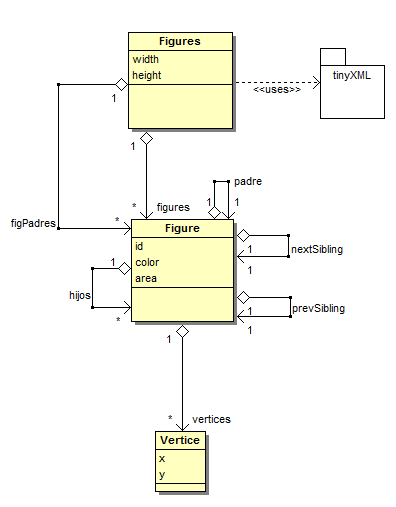
\includegraphics[scale=0.60]{graphics/diagramaClasesFigure.png}
		\caption{Diagrama de clases de la estructura de datos \emph{Figuras}}
		\label{fig:diagramaClasesFigure}
		\end{figure}
		
	Como se puede ver, se ha implementado mediante tres clases principales más una librería externa:
	
	\begin{itemize}
	
		\item \textbf{Figures:} Almacena la lista de figuras presentes en la imagen, permite manipular y acceder a ellas tanto en forma de lista (colocándose todas las figuras existentes de forma seguida y sin jerarquías) como en forma de árbol (jerarquizándolas según quién está dentro de quién: una figura que contiene en su interior todos los vértices de otra será su ``padre''), ocupándose de forma autosuficiente de mantener ésta última estructura al añadir nuevas figuras.\\

		Además posee también funcionalidad para guardar y cargar su información en formato XML, así como para eliminar figuras repetidas o volver a calcular el color de cada figura teniendo en cuenta las figuras que contiene (ver Sección~\ref{sec:algAnalisis} para más detalles sobre estas funcionalidades).
		
		\item \textbf{Figure:} Representa cada elemento almacenado en la clase Figures. Contiene, como nodo de la estructura arbórea creada en Figures, los atributos necesarios para referenciar a sus padres, sus hijos y sus hermanos, y como elemento representativo de una figura en la imagen (Sección~\ref{subsec:xmlstruct}), el color, area y lista de vértices correspondiente a la imagen.\\
		
		Presenta métodos para poder acarrear funciones geométricas básicas (como transformar su representación de vértices de coordenadas cartesianas a euclídeas) que simplifican el desarrollo de los algoritmos explicados en la Sección~\ref{sec:algComposicion}.
		
		\item \textbf{Vertice:} Se trata de la unidad más pequeña de esta estructura, y representa las coordenadas en 2 dimensiones de un vértice en el plano cartesiano. Como se detalla en la Sección~\ref{subsec:xmlstruct}, da la opción de ser considerado un ``centro'', de forma que, en la lista de vértices de la Figura que lo almacene, puede actuar como el centro entre el vértice anterior y el siguiente, formando por tanto un arco entre los 3 vértices y permitiendo realizar curvas en las figuras.
		
		\item \textbf{TinyXML:} Se trata de un paquete externo de código libre que permite generar y manipular archivos XML.
	
	\end{itemize}
	
			
\subsection{Usos de la estructura}	
\label{subsec:usosFigure}

	Como ya se ha comentado, tanto el proceso de análisis como el de composición hacen uso de esta estructura y, dado que para la implementación de ambos módulos se ha seleccionado el mismo lenguaje orientado a objetos (C++), estos compartirán la implementación de esta estructura.\\
	
	Sin embargo, existen diferencias entre los usos y ampliaciones que cada módulo aplica, y es por eso que no hacen uso de la estructura de forma directa,  sino que cada módulo heredará la clase \emph{Figure} para satisfacer sus propias necesidades. El resultado es el diagrama mostrado en la Figura~\ref{fig:diagramaFigMupPhic}, con diferenciación entre \emph{FigureImg} y \emph{FigureMusic}.\\

		\begin{figure}[htbp]
		\centering
		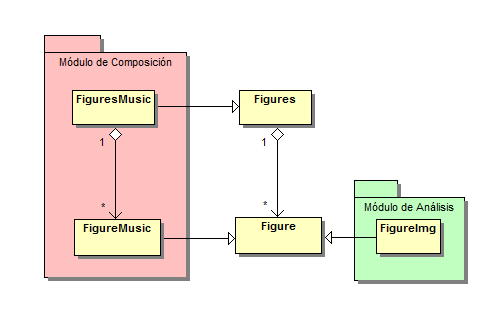
\includegraphics[scale=0.5]{graphics/diagramaFigMupPhic.png}
		\caption{Diagrama de clases de los diferentes tipos de Figura}
		\label{fig:diagramaFigMupPhic}
		\end{figure}
		
	Los detalles de cada clase hija serán explicados en posteriores secciones.	


\section{Formato de representación de música}
\label{sec:repMusic}

\gotrev{Última revisión hecha el 20-06-2012}

La estructura para representar la música propuesta en el proyecto está determinada por un árbol que trabaja desde el elemento más general, la canción que se va a componer, al más específico, cada una de las notas que componen dicha canción. Se puede ver la estructura en el siguiente esquema (Figura~\ref{fig:structmusic}).\\
	
	\begin{figure}[htbp]
	\centering
	\hspace*{-0.1in}
	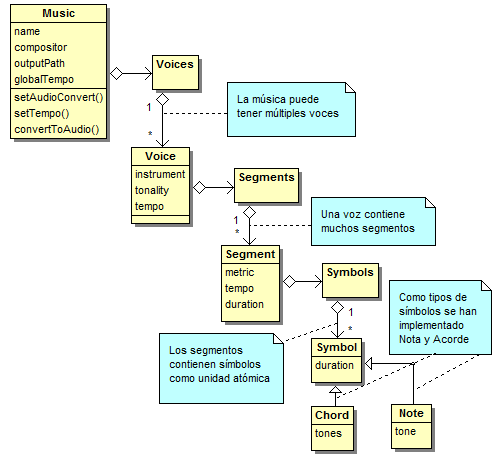
\includegraphics[scale=0.6]{graphics/musica-estructura.png}
	\caption{Estructura de datos de una pieza musica}
	\label{fig:structmusic}
	\end{figure}


\textbf{Music}: Al nivel de la Music trabajamos con la información relativa a toda la canción que se va a componer. Por un lado está la información relativa al nombre de la pieza y del compositor que la ha hecho así como la ruta del archivo de sonido cuando se guarde. Pero la parte más importante es el contenido de las voces a partir de las cuales está formada la canción. También es importante el tempo global de la pieza y la herramienta que se usará para crear el archivo de audio de salida.
\newline

\textbf{Voices}: Esta clase es un envoltorio de un array al que se le ha añadido pequeña funcionalidad, como la posibilidad de editar algún parámetro a todas las voces que contiene.
\newline

\textbf{Voz}: Por debajo de Music se trabaja con las voces, Voice. Dentro de cada Voice se determina el instrumento, la tonalidad y el tempo con el que será transformada esta voz en sonido. La parte sustancial de cada voz son los Segments, donde se almacena los datos musicales.
\newline

\textbf{Segments}: Al igual que Voices, es un envoltorio de un array al que se le ha añadido alguna pequeña funcionalidad adicional.
\newline

\textbf{Segment}: Su principal cometido es almacenar de forma serializable los diferentes símbolos musicales de los que está compuesta la pieza musical. A su vez, estos elementos tienen la posibilidad de establecer su propia métrica y tempo. Además es importante la duración del segmento, que se irá incrementando cada vez que se añada un nuevo símbolo.
\newline

\textbf{Symbol}: Son la unidad a partir de la cual se crean todos los elementos básicos de la música, Symbol está formado únicamente por una duración. Actualmente se ha desarrollado dos tipos de elementos a partir de Symbol:
\begin{itemize}

	\item \textbf{Note}: Estos símbolos tienen asociado además de duración, determinada por el componente anterior, un tono que viene representado por un número que posteriormente será interpretado con la herramienta que generará el archivo de audio.

	\item \textbf{Chord}: Los acordes están formados de la misma manera que las notas, pero en lugar de tener asociado un único tono pueden tener de dos a cuatro tonos diferentes. En la práctica, esto se traduce a varios tonos sonando a la vez durante el mismo tiempo dentro de la pieza musical sin la necesidad de múltiples voces.

\end{itemize}
 
